% ----------------------------------------------------
\begin{frame}
  \titlepage
\end{frame}
% ----------------------------------------------------
\note{Última sesión magistral del curso. En lugar de recorrer temas nuevos, hoy cerramos con cinco grandes debates de la política mundial de 2026. Cada debate es una oportunidad para aplicar el marco analítico del curso (intereses, interacciones, instituciones) a problemas reales. Al final de la clase deberían poder coger cualquier titular de prensa y analizarlo con las herramientas que hemos construido durante el cuatrimestre.}

% ----------------------------------------------------
\begin{frame}
\frametitle{Hoy: cinco grandes debates}
\centering
\vspace{1em}
\begin{enumerate}
  \setlength{\itemsep}{8pt}
  \item ¿Vuelve la guerra entre grandes potencias?
  \item ¿Puede el mundo cooperar ante bienes públicos globales?
  \item ¿Es reversible la globalización?
  \item ¿Sigue funcionando el orden liberal?
  \item Nuevas fronteras: nuclear, cyber, IA
\end{enumerate}

% \vspace{1em}
% \small Cierre: todo conecta, Intereses--Interacciones--Instituciones
\end{frame}
% ----------------------------------------------------
\note{Presentar la estructura de la clase. No son cinco bloques independientes: están entrelazados. El ascenso de China toca todos los debates. El clima conecta con el debate sobre cooperación y con el orden liberal. La guerra en Ucrania aparece en casi todos. Invitar a los estudiantes a ir identificando conexiones entre debates a medida que avanzamos.}

% % ----------------------------------------------------
% \begin{frame}
% \frametitle{Recordatorio: el marco del curso}
% \centering
% \vspace{0.5em}

% \begin{columns}[T]
% \begin{column}{0.32\textwidth}
% \centering
% \textcolor{accent}{\textbf{Intereses}}\\[4pt]
% \scriptsize ¿Qué quieren los actores?\\
% Poder, seguridad, riqueza, ideología
% \end{column}
% \begin{column}{0.32\textwidth}
% \centering
% \textcolor{accent2}{\textbf{Interacciones}}\\[4pt]
% \scriptsize ¿Cómo se relacionan?\\
% Cooperación, conflicto, negociación
% \end{column}
% \begin{column}{0.32\textwidth}
% \centering
% \textcolor{accent}{\textbf{Instituciones}}\\[4pt]
% \scriptsize ¿Qué reglas los moldean?\\
% ONU, OMC, alianzas, normas
% \end{column}
% \end{columns}

% \vspace{1.5em}
% \small\textit{Los cinco debates de hoy se pueden leer con estas tres lentes}
% \end{frame}
% % ----------------------------------------------------
% \note{Volver al marco I--I--I (Frieden, Lake, Schultz) que vimos en el tema 2. Todos los debates de hoy son combinaciones de estos tres elementos:
% \begin{itemize}
%   \item Intereses: qué quieren los actores y cómo se distribuyen las preferencias (domésticas e internacionales)
%   \item Interacciones: modelos de negociación, dilemas de cooperación, acción colectiva
%   \item Instituciones: reglas formales (tratados, OOII) e informales (normas)
% \end{itemize}
% Este marco es lo más importante que se llevan del curso. Los debates concretos cambiarán en cinco años; el marco sirve para analizar los que vengan.}

% ====================================================
\section{¿Vuelve la guerra entre grandes potencias?}
% ====================================================

% ----------------------------------------------------
\begin{transitionframe}
¿Vuelve la guerra entre grandes potencias?
\end{transitionframe}
% ----------------------------------------------------
\note{}

% ----------------------------------------------------
\begin{frame}
\centering
\vspace{2em}
{\large Desde 1945, \textbf{ninguna guerra directa} entre grandes potencias.\\[10pt]
Fin de ese período excepcional?}
\end{frame}
% ----------------------------------------------------
\note{Plantear el debate. La ``larga paz'' entre grandes potencias (Gaddis) es una anomalía histórica: 80 años sin que EE.UU., Rusia/URSS, China, Reino Unido o Francia se enfrenten directamente. Antes de 1945, era habitual cada pocas décadas. Hoy, con Ucrania, Taiwán y la rivalidad EEUU--China, esa excepción empieza a cuestionarse. No hablamos de guerra directa nuclear sino de escenarios donde grandes potencias se enfrentan en terceros países o indirectamente.}

% ----------------------------------------------------
\begin{frame}
\frametitle{Ucrania: la guerra interestatal ha vuelto a Europa}
\centering

\begin{itemize}
  \item<1-> \textbf{Febrero 2022:} Rusia invade Ucrania --- mayor guerra en Europa desde 1945
  \vspace{6pt}
  \item<2-> Desafía tres supuestos del orden de posguerra:
  \begin{itemize}
    \item Soberanía e integridad territorial
    \item Interdependencia económica $\neq$ paz
    \item (No tanto) Disuasión nuclear, amenazas explícitas
  \end{itemize}
  \vspace{6pt}
  \item<3-> Respuesta: \textbf{sanciones} sin precedentes (SWIFT, reservas)
  \item<4-> 2026: la guerra continúa, con un frente estancado y negociaciones intermitentes
\end{itemize}
\end{frame}
% ----------------------------------------------------
\note{Ucrania es el caso más claro de que la guerra interestatal no es cosa del pasado. Es también un desafío directo al orden liberal de posguerra construido tras 1945: Rusia viola el principio más básico (soberanía) y lo hace usando amenazas nucleares. La teoría liberal predecía que la interdependencia económica (Rusia era el principal proveedor de gas de Europa) haría imposible la guerra. No fue así. Farrell y Newman (tema 08): la interdependencia no solo puede fallar como mecanismo de paz, sino que puede ser instrumentalizada. Las sanciones a Rusia son el mayor caso de weaponized interdependence de la historia.}

% ----------------------------------------------------
\begin{frame}
\frametitle{Trump II}
\centering

\begin{itemize}
  \item<1-> \textbf{Nueva estrategia (sept 2025)}: \textit{National Defense Strategy} en sept 2025, seguridad doméstica, Monroe
  \item<2-> \textbf{Ataque a internacionalismo:} USAID, OMS/WHO, ONU
  \item<3-> \textbf{Amenazas:} Groenlandia, OTAN, canal de Panamá...
  \vspace{5pt}
  \item<4-> \textbf{Venezuela:} despliegue militar en el Caribe, captura de Maduro
  \item<5-> \textbf{Irán:} Operación\ \textit{Epic Fury} junto a Israel, caos global
  \vspace{6pt}
  \item<5-> \alert{El garante del orden liberal internacional está reventándolo desde dentro}
\end{itemize}
\end{frame}
% ----------------------------------------------------
\note{Si Ucrania mostró el desafío externo al orden liberal, la segunda administración Trump muestra el desafío interno: el propio hegemón actuando como potencia revisionista. Caribe: tras meses de despliegue naval y ataques a embarcaciones acusadas de narcotráfico, fuerzas especiales capturan a Maduro en enero de 2026 y lo trasladan a EE.UU. Oriente Medio: tras declarar fracasadas las negociaciones nucleares, EE.UU. e Israel lanzan ataques coordinados contra Irán el 28 de febrero; un ataque al complejo presidencial en Teherán mata a Jamenei; Irán responde contra bases de EE.UU. en la región. A esto se suman amenazas reiteradas de uso de la fuerza para anexionar Groenlandia, retomar el Canal de Panamá, o intervenir en Colombia y México. Y la retirada de instituciones multilaterales: OMS, recortes drásticos a USAID y agencias de la ONU. Conexión teórica clave: el orden liberal no solo se ve amenazado por outsiders (Rusia, China); el propio hegemón que lo construyó cuestiona sus reglas. Es una lección sobre la fragilidad de los órdenes internacionales cuando el patrocinador deja de querer pagar el coste.}

% ----------------------------------------------------
\imageframe{../img/solar_exports_china.png}
\note{}
% ----------------------------------------------------
  
% ----------------------------------------------------
\begin{frame}
\frametitle{Taiwán: el siguiente punto de fricción}
\centering

\begin{itemize}
  \item<1-> \textbf{Taiwán:} democracia de facto, reclamada por China como provincia
  \vspace{6pt}
  \item<2-> ¿Por qué importa tanto?
  \begin{itemize}
    \item TSMC produce $\sim$90\% de los \textbf{semiconductores avanzados} mundiales
    \item Posición estratégica en el Pacífico occidental
    \item Símbolo político: democracia china viable
  \end{itemize}
  \vspace{6pt}
  \item<3-> EE.UU.: ``\textbf{ambigüedad estratégica}'' --- ni promete ni niega la defensa
  \vspace{6pt}
  \item<4-> \alert{El detonante} más plausible de una guerra EE.UU.--China
\end{itemize}
\end{frame}
% ----------------------------------------------------
\note{Taiwán concentra todos los ingredientes de una crisis. Económicamente: TSMC es el nodo crítico de la cadena global de semiconductores; una interrupción paralizaría la economía mundial. Militarmente: está a 160 km de la costa china, en el centro de la primera cadena de islas del Pacífico. Políticamente: su democratización desde los años 90 la convierte en un modelo que China no puede tolerar. EE.UU. mantiene desde 1979 una ambigüedad estratégica: vende armas a Taiwán pero no garantiza formalmente su defensa. El objetivo es disuadir a China y a la vez evitar que Taiwán declare independencia. En los últimos años Biden rompió varias veces esa ambigüedad diciendo que EE.UU. defendería la isla; la administración actual oscila. Este es probablemente el punto donde el modelo de bargaining (tema 03) tiene más riesgo de fallar: los problemas de compromiso son agudos, el bien es casi indivisible.}

% ----------------------------------------------------
\begin{frame}
\frametitle{La trampa de Tucídides: EE.UU.--China}
\centering

\begin{itemize}
  \item<1-> \textbf{Transición de poder:} potencia emergente $\to$ potencia dominante
  \item<2-> Graham Allison (2017): 16 casos históricos, 12 acabaron en guerra
  \vspace{6pt}
  \item<3-> \textcolor{accent}{Factores que empujan al conflicto:}
  \begin{itemize}
    \item Guerra preventiva del hegemón
    \item Revisionismo del emergente
    \item Nacionalismo doméstico en ambos
  \end{itemize}
  \vspace{6pt}
  \item<4-> \textcolor{accent2}{Factores que frenan:}
  \begin{itemize}
    \item Armas nucleares (MAD)
    \item Interdependencia económica
    \item Instituciones internacionales
  \end{itemize}
\end{itemize}
\end{frame}
% ----------------------------------------------------
\note{La teoría de la transición de poder (Organski; Gilpin) aplicada al caso más importante del siglo XXI. Allison estudió 16 transiciones de poder en 500 años; 12 acabaron en guerra. El paralelo con Atenas--Esparta da nombre al concepto. Pero no estamos condenados: los cuatro casos pacíficos de Allison tenían instituciones fuertes, comunicación, y reconocimiento mutuo. El bargaining model nos dice que la guerra es siempre costosa e ineficiente; ocurre cuando hay información incompleta, problemas de compromiso o indivisibilidad. EE.UU.--China tienen los tres: desconfianza mutua creciente, dudas sobre compromisos futuros (Taiwán), y algunos bienes son difíciles de dividir.}

% ----------------------------------------------------
\begin{frame}
\frametitle{Vuelve la guerra?}
\centering

\begin{columns}[T]
\begin{column}{0.47\textwidth}
\textcolor{accent2}{\textbf{Sí}}
\begin{itemize}
  \setlength{\itemsep}{5pt}
  \item Ucrania, Oriente Medio
  \item Rearme global acelerado
  \item Nacionalismo en auge
  \item Instituciones debilitadas
  \item Taiwán como polvorín
  \item Nuevas tecnologías? (drones, AI)
\end{itemize}
\end{column}
\begin{column}{0.47\textwidth}
\textcolor{accent}{\textbf{No}}
\begin{itemize}
  \setlength{\itemsep}{5pt}
  \item MAD sigue funcionando
  \item Comercio EEUU--China
  \item Sin guerra directa en 80 años
  \item Costes económicos prohibitivos
  \item Canales de comunicación activos
\end{itemize}
\end{column}
\end{columns}

\vspace{10pt}
\onslide<2->{\centering\small \textit{Reminder: clase sobre bargaining, alianzas, paz democrática, etc}}
\end{frame}
% ----------------------------------------------------
\note{Balance del debate. Argumentos a favor: Ucrania muestra que el tabú de la guerra interestatal se ha roto; el gasto militar global alcanza máximos de la Guerra Fría; la retórica nacionalista aumenta en EEUU, China, Rusia, India; ONU y OMC están cada vez más paralizadas. Argumentos en contra: las condiciones estructurales que mantuvieron la paz (nucleares, interdependencia, instituciones) siguen ahí; EEUU y China comercian por casi 700.000 millones al año; los costes de una guerra serían astronómicos. La respuesta más honesta: la probabilidad de guerra directa sigue siendo baja, pero más alta que hace 20 años. El riesgo real no es una guerra deliberada sino una escalada accidental (Taiwán, Mar de China Meridional).}

% ====================================================
\section{¿Puede el mundo cooperar ante bienes públicos globales?}
% ====================================================

% ----------------------------------------------------
\begin{transitionframe}
¿Puede el mundo cooperar ante bienes públicos globales?
\end{transitionframe}
% ----------------------------------------------------
\note{}

% ----------------------------------------------------
\begin{frame}
\centering
\vspace{2em}
{\large El clima, las pandemias, la biodiversidad\dots\\[10pt]
Problemas que afectan a todos, pero donde \textbf{cada uno tiene incentivos para no pagar}}
\end{frame}
% ----------------------------------------------------
\note{Planteamiento del debate. Los bienes públicos globales son el caso más puro del dilema de la cooperación internacional. Todos nos beneficiamos del aire limpio, la estabilidad climática, la contención de patógenos. Pero nadie puede ser excluido y el consumo es no rival: condiciones perfectas para el free-riding.}

% ----------------------------------------------------
\begin{frame}
\frametitle{La tragedia de los comunes}
\centering
\vspace{0.5em}

\resizebox{0.75\textwidth}{!}{%
\begin{tikzpicture}[>=stealth, thick]
  \node[draw, fill=accent!20, rounded corners, minimum width=3cm, minimum height=1.5cm, align=center] (res) at (0,0) {\textbf{Recurso común}\\\small (atm\'osfera, oc\'eano)};
  \node[draw, circle, fill=accent2!15, minimum size=1.1cm, align=center, font=\small] (a1) at (-4, 2) {Estado\\A};
  \node[draw, circle, fill=accent2!15, minimum size=1.1cm, align=center, font=\small] (a2) at (0, 3) {Estado\\B};
  \node[draw, circle, fill=accent2!15, minimum size=1.1cm, align=center, font=\small] (a3) at (4, 2) {Estado\\C};
  \node[draw, circle, fill=accent2!15, minimum size=1.1cm, align=center, font=\small] (a4) at (-3, -2.5) {Empresa\\X};
  \node[draw, circle, fill=accent2!15, minimum size=1.1cm, align=center, font=\small] (a5) at (3, -2.5) {Empresa\\Y};
  \draw[->, accent2, thick] (res) -- (a1);
  \draw[->, accent2, thick] (res) -- (a2);
  \draw[->, accent2, thick] (res) -- (a3);
  \draw[->, accent2, thick] (res) -- (a4);
  \draw[->, accent2, thick] (res) -- (a5);
  \node[font=\small\itshape, text=asher] at (0, -3.8) {Cada actor se beneficia; el recurso se agota};
\end{tikzpicture}}
\end{frame}
% ----------------------------------------------------
\note{Hardin (1968). Cada actor tiene incentivos individuales para sobreexplotar. Lo vimos en el tema sobre comercio y en el libro FLS cap.~13: el clima es un dilema del prisionero repetido con 193 jugadores. Ostrom (Nobel 2009) mostró que comunidades locales pueden gestionar comunes sin Estado ni privatización, pero a escala global es mucho más difícil: faltan mecanismos de monitorización y sanción.}

% ----------------------------------------------------
\begin{frame}
\frametitle{¿Qué facilita la cooperación?}
\centering

\begin{itemize}
  \item<1-> \textbf{Pocos actores} $\to$ más fácil coordinar
  \item<2-> \textbf{Problema simple} con sustitutos disponibles
  \item<3-> \textbf{Interacción repetida} (sombra del futuro)
  \item<4-> \textbf{Productos conjuntos} (\textit{joint products}, beneficios adicionales)
  \item<5-> \textbf{Grupo privilegiado} (líder dispuesto a pagar)
\end{itemize}

\vspace{10pt}
\onslide<6->{\small \textcolor{accent}{Protocolo de Montreal (1987)} sobre la capa de ozono, cumplía los cinco.\\El \textcolor{accent2}{clima} con suerte, solo el tercero}
\end{frame}
% ----------------------------------------------------
\note{Los cinco factores de FLS cap.~13. Montreal fue un éxito: pocos productores de CFC, sustituto disponible (DuPont), ciencia clara, EEUU como líder, fondo para países en desarrollo. El clima es lo contrario: 193 países, toda la economía implicada, costes inmediatos vs. beneficios lejanos, asimetría entre contaminadores y víctimas, sin liderazgo estable.}

% ----------------------------------------------------
\begin{frame}
\frametitle{Acuerdo de París: 10 años después}
\centering

\begin{itemize}
  \item<1-> \textbf{2015:} objetivo de limitar el calentamiento a 1{,}5--2\textdegree C
  \item<2-> Mecanismo: contribuciones voluntarias (NDCs), revisión cada 5 años
  \vspace{6pt}
  \item<3-> \textcolor{accent}{Logro:} casi universal (195 partes)
  \item<4-> \textcolor{accent2}{Límite:} sin mecanismo de cumplimiento vinculante
  \vspace{6pt}
  \item<5-> \textbf{2026:} las trayectorias actuales apuntan a $\sim$2{,}5--3\textdegree C
  \item<6-> Salida y reentrada de EE.UU. (Trump--Biden--Trump\dots)
\end{itemize}
\end{frame}
% ----------------------------------------------------
\note{El Acuerdo de París cumple 10 años. La genialidad: siendo voluntario, consiguió adhesión casi universal. La debilidad: siendo voluntario, nadie está obligado. Diez años después, las emisiones globales siguen subiendo en términos absolutos, aunque la intensidad energética baja. La reentrada/salida de EEUU ha minado la credibilidad del régimen. Conexión con la sesión de derecho internacional (tema 06): ¿puede el derecho blando ser efectivo? Depende de presión social, finanzas (desinversión en fósiles) y tecnología (si renovables son rentables sin subsidios).}

% ----------------------------------------------------
\begin{frame}
\frametitle{La tensión Norte--Sur}
\centering
\vspace{0.5em}

% \resizebox{0.78\textwidth}{!}{%
% \begin{tikzpicture}[>=stealth, thick]
%   \node[draw, fill=accent!20, rounded corners, minimum width=3.5cm, minimum height=2cm, align=center] (north) at (-3.5,0) {\textbf{Norte global}\\\small Responsables\\\scriptsize emisiones hist\'oricas};
%   \node[draw, fill=accent2!15, rounded corners, minimum width=3.5cm, minimum height=2cm, align=center] (south) at (3.5,0) {\textbf{Sur global}\\\small Sufre m\'as\\\scriptsize pero necesita crecer};
%   \draw[<->, very thick, accent2] (north) -- (south) node[midway, above, font=\small\bfseries] {Tensi\'on};
%   % \node[font=\scriptsize\itshape, text=asher, align=center] at (0, -1.3) {``¿Por qu\'e limitar nuestro desarrollo\\por un problema que vosotros causasteis?''};
%   \node[draw, fill=accent!10, rounded corners, font=\small, align=center] at (0, -2.9) {\textbf{Responsabilidades comunes pero diferenciadas}};
% \end{tikzpicture}}

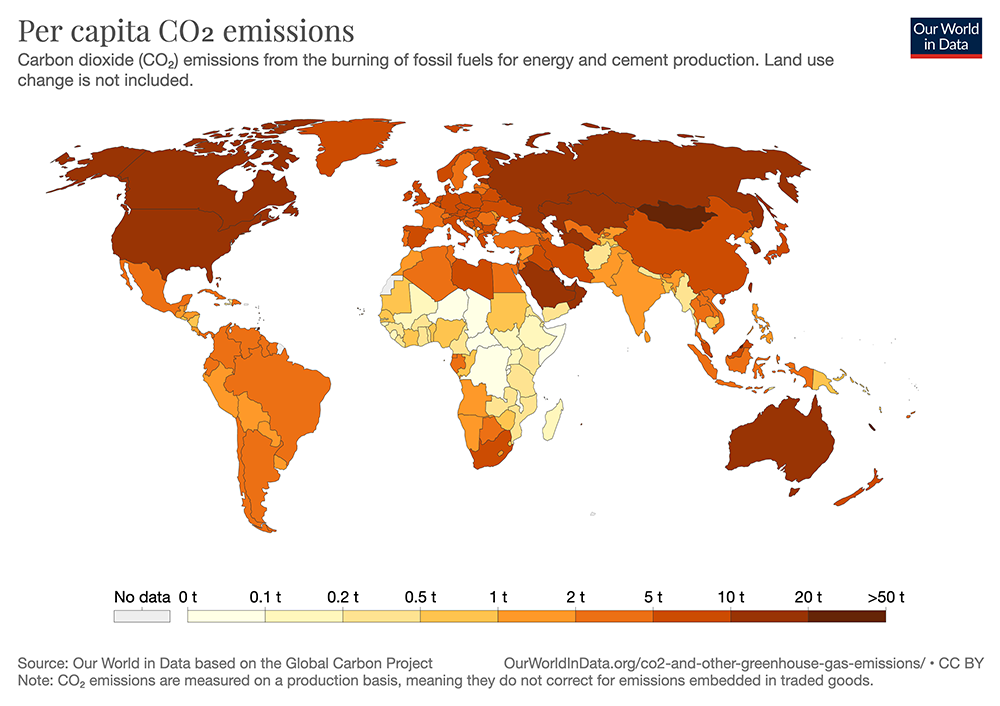
\includegraphics[width = \textwidth]{../img/emissions_per_capita}

\end{frame}
% ----------------------------------------------------
\note{La tensión Norte--Sur es central. EEUU per cápita emite $\sim$15 toneladas de CO2; India $\sim$2. ¿Es justo pedir a India que limite su crecimiento por un problema que causaron los ricos? El principio de responsabilidades comunes pero diferenciadas intenta resolver esto: todos actúan, pero los ricos más y primero. En la práctica se traduce en financiación climática (100.000 millones anuales prometidos, parcialmente cumplidos). Esta tensión explica por qué las COP son tan lentas y por qué cada año el conflicto se traslada a un tema distinto (mitigación, adaptación, pérdidas y daños).}

% ----------------------------------------------------
\begin{frame}
\frametitle{Más allá del clima: pandemias}
\centering

\begin{itemize}
  \item<1-> COVID-19: $\sim$7 millones de muertes confirmadas, $\sim$15--25 millones estimadas
  \vspace{6pt}
  \item<2-> Lecciones para la cooperación global:
  \begin{itemize}
    \item Nacionalismo de vacunas
    \item COVAX subfinanciado
    \item OMS con pocos recursos y autoridad
  \end{itemize}
  \vspace{6pt}
  \item<3-> 2024: \textbf{Acuerdo sobre pandemias} en la OMS\dots aún parcial y sin compromisos vinculantes
  \vspace{6pt}
  \item<4-> \alert{Cuando llegue la próxima?}
\end{itemize}
\end{frame}
% ----------------------------------------------------
\note{Las pandemias son el otro gran bien público global. COVID-19 mostró lo mismo que el clima: los incentivos colectivos y los individuales divergen. Los países ricos acapararon vacunas, la OMS tiene poco poder real, COVAX cubrió una fracción de la población de países pobres. El acuerdo pandémico de la OMS, negociado tras la pandemia, ha avanzado con mucha resistencia. Conexión con el curso: mismo problema estructural que el clima (bien público global, free-riding, asimetrías). Las herramientas conceptuales son idénticas aunque el dominio cambie.}

% ----------------------------------------------------
\begin{frame}
\frametitle{Puede el mundo cooperar?}
\centering

\begin{columns}[T]
\begin{column}{0.47\textwidth}
\textcolor{accent}{\textbf{Sí}}
\begin{itemize}
  \setlength{\itemsep}{5pt}
  \item Montreal funcionó
  \item Renovables ya más baratas
  \item China lidera solar y baterías
  \item Interacción repetida (COP)
\end{itemize}
\end{column}
\begin{column}{0.47\textwidth}
\textcolor{accent2}{\textbf{No}}
\begin{itemize}
  \setlength{\itemsep}{5pt}
  \item 193 actores asimétricos
  \item Sin sanciones creíbles
  \item Costes inmediatos, beneficios lejanos
  \item Política doméstica (Olson)
\end{itemize}
\end{column}
\end{columns}

\vspace{10pt}
\onslide<2->{\centering\small \textit{Reminder: clase sobre normas internacionales}}
\end{frame}
% ----------------------------------------------------
\note{Balance del debate:
\begin{itemize}
  \item Optimistas: Montreal demuestra que se puede; la transición energética avanza sola por razones de mercado; la acción no estatal (ciudades, empresas) complementa la estatal
  \item Pesimistas: el clima es mucho más complejo que el ozono; la política doméstica bloquea la acción (Olson: los contaminadores son pocos y organizados, los beneficiarios muchos y dispersos); sin sanciones, el free-riding es inevitable
\end{itemize}
La respuesta matizada: la cooperación es posible pero lenta e incompleta. Probablemente llegaremos a 2--2{,}5\textdegree C, no a 1{,}5\textdegree C. Eso no es un fracaso total pero tampoco un éxito.}

% ====================================================
\section{¿Es reversible la globalización?}
% ====================================================

% ----------------------------------------------------
\begin{transitionframe}
¿Es reversible la globalizaci\'on?
\end{transitionframe}
% ----------------------------------------------------
\note{}

% ----------------------------------------------------
\begin{frame}
\centering
\vspace{2em}
{\large Aranceles, sanciones, \textit{decoupling}, \textit{friendshoring}\dots\\[10pt]
¿Estamos desmontando medio siglo de integraci\'on econ\'omica?}
\end{frame}
% ----------------------------------------------------
\note{Planteamiento del debate. Desde los años 80, la globalización parecía imparable: caída de aranceles, cadenas de valor globales, flujos financieros masivos. Desde 2016 (Brexit, Trump I) y sobre todo desde 2018 (guerra comercial EEUU--China), el proceso parece revertirse. La pregunta: ¿es un bache o un cambio estructural?}

% ----------------------------------------------------
\begin{frame}
\frametitle{La globalización en cifras}
\centering

\begin{itemize}
  \item<1-> \textbf{Comercio/PIB mundial:} $\sim$25\% en 1970 $\to$ $\sim$60\% en 2008 $\to$ estancado desde entonces
  \vspace{6pt}
  \item<2-> \textbf{Inversión extranjera directa:} cae desde máximos de 2015
  \vspace{6pt}
  \item<3-> \textbf{Aranceles:} EEUU a China, $\sim$3\% en 2017 $\to$ $\sim$20\% en 2020 $\to$ y los aranceles de Trump en 2025
  \vspace{6pt}
  \item<4-> \textbf{Sanciones activas:} Rusia, Irán, NK, China tech
\end{itemize}

% \vspace{8pt}
% \onslide<4->{\small ``Slowbalisation'' o ``\textit{deglobalization}'': el debate está abierto}
\end{frame}
% ----------------------------------------------------
\note{Los datos son ambiguos. El ratio comercio/PIB mundial creció casi sin parar hasta 2008 y desde entonces está plano. No es retroceso drástico, pero sí fin del impulso. La IED cae. Los aranceles suben. Las sanciones proliferan: más de 20.000 entidades sancionadas en todo el mundo. Algunos autores hablan de ``slowbalisation'' (ralentización); otros de ``deglobalization'' (reversión). Lo importante para el curso: los flujos cambian no solo en cantidad sino en dirección (más entre aliados, menos entre rivales).}

% ----------------------------------------------------
\begin{frame}
\frametitle{\textit{Decoupling} EE.UU.--China}
\centering

\begin{itemize}
  \item<1-> \textbf{Guerra comercial 2018:} aranceles Trump, represalias chinas
  \item<2-> \textbf{Tecnología 2022--2026:} CHIPS Act, restricciones a ASML/NVIDIA
  \item<3-> \textbf{Caos de 2025:} Liberation Day tariffs
  \item[]<3-> (No es la misma motivación)
  \vspace{6pt}
  \item<4-> Tensión actual sobre semiconductores, IA, quantum computing, etc
\end{itemize}
\end{frame}
% ----------------------------------------------------
\note{El decoupling real es selectivo, no total. En bienes de consumo, EEUU y China siguen profundamente integrados; EEUU depende de China para muchos insumos. En tecnología avanzada (semiconductores <7nm, equipos de litografía, IA), sí hay separación activa. La CHIPS Act de 2022 y las restricciones a ASML (Países Bajos) y NVIDIA materializan lo que Farrell y Newman llaman weaponized interdependence: usar los nodos críticos de la red global como arma. Conexión con tema 08: los flujos financieros y tecnológicos se instrumentalizan geopolíticamente.}

% ----------------------------------------------------
\begin{frame}
\frametitle{Sanciones: el instrumento preferido}
\centering

\begin{itemize}
  \item<1-> \textbf{Rusia 2022:} mayor régimen de sanciones de la historia
  \begin{itemize}
    \item Exclusión del SWIFT, congelación de $\sim$300.000 M\$ en reservas
  \end{itemize}
  \vspace{6pt}
  \item<2-> ¿Funcionan las sanciones?
  \begin{itemize}
    \item Dañan la economía rusa, pero no detuvieron la guerra
    \item Rusia redirigió exportaciones a China e India
    \item Surgimiento de sistemas de pago alternativos
  \end{itemize}
  \vspace{6pt}
  \item<3-> \alert{Riesgo no intencionado:} acelerar la \textbf{desdolarización} y crear bloques
  \item[]<3-> La weaponized interdependence es en parte un arma de un sólo uso. Y si hay conflicto... Hormuz y el Petroyuan
\end{itemize}
\end{frame}
% ----------------------------------------------------
\note{Las sanciones son la herramienta geopolítica de moda. Rusia en 2022 es el caso más extremo: congelación de reservas del banco central, exclusión de SWIFT, sanciones secundarias. Funcionaron parcialmente: la economía rusa se contrajo, pero la guerra sigue. Además, las sanciones tienen un efecto no deseado: empujan a actores a construir alternativas. China ha acelerado CIPS (alternativa a SWIFT); BRICS discuten monedas alternativas al dólar. Hudson Bay, Stuenkel y otros argumentan que el uso masivo de sanciones puede erosionar el privilegio exorbitante del dólar a medio plazo. Conexión con tema 08 (finanzas internacionales).}

% ----------------------------------------------------
\begin{frame}
\frametitle{\textit{Friendshoring} y nueva geografía productiva}
\centering

\begin{itemize}
  \item<1-> \textbf{Friendshoring:} mover cadenas de valor a países ``amigos''
  \item<2-> \textbf{Nearshoring:} acercar la producción al mercado (México para EEUU)
  \vspace{6pt}
  \item<3-> Ejemplos 2023--2026:
  \begin{itemize}
    \item Apple: parte de producción India y Vietnam
    \item TSMC: nuevas fábricas en EEUU, Japón, Alemania
    \item IED récord en México y Vietnam
  \end{itemize}
  \vspace{6pt}
  \item<4-> \textit{No} es desglobalización: es \textbf{reconfiguración} según bloques geopolíticos
\end{itemize}
\end{frame}
% ----------------------------------------------------
\note{El friendshoring (Janet Yellen, 2022) es la propuesta de que las cadenas de valor se reorganicen según alianzas políticas y no solo según costes. México, Vietnam, India, Polonia son los grandes beneficiarios. Esto no es desglobalización: es globalización segmentada. Las cadenas siguen siendo transfronterizas, pero dentro de bloques. Conexión con tema 07 (comercio): los modelos clásicos (Ricardo, H--O) predicen que esto reduce eficiencia; los modelos de economía política explican por qué los Estados aceptan ese coste por seguridad.}

% ----------------------------------------------------
\begin{frame}
\frametitle{El fin de la globalización?}
\centering

\begin{columns}[T]
\begin{column}{0.47\textwidth}
\textcolor{accent2}{\textbf{Sí}}
\begin{itemize}
  \setlength{\itemsep}{5pt}
  \item Aranceles récord
  \item Sanciones masivas
  \item Decoupling tecnológico
  \item Industrial policy (CHIPS, IRA)
  \item Fin del ``consenso de Washington''
  \item Trump II y bloques geopolíticos
\end{itemize}
\end{column}
\begin{column}{0.47\textwidth}
\textcolor{accent}{\textbf{No}}
\begin{itemize}
  \setlength{\itemsep}{5pt}
  \item Comercio total sigue alto
  \item Servicios y datos crecen
  \item Friendshoring $\neq$ autarquía
  \item Intereses empresariales presionan
  \item Costes políticos altos
\end{itemize}
\end{column}
\end{columns}

\vspace{10pt}
\onslide<2->{\centering\small \textit{Reminder: comercio, finanzas, weaponized interdependence, etc}}
\end{frame}
% ----------------------------------------------------
\note{Balance. La globalización no se está revirtiendo de forma lineal: se está transformando. Las cadenas se reorganizan por bloques; los flujos de bienes físicos se ralentizan pero los de datos y servicios siguen creciendo. Los intereses domésticos son contradictorios: las empresas quieren acceso a China; los gobiernos quieren reducir dependencia. Ejemplo claro en el curso: las industrias que presionaron por el libre comercio en los 90 son hoy las que presionan por subsidios industriales. El modelo de economía política (tema 07) predice exactamente eso: cuando cambian los ganadores y perdedores, cambia la política.}

% ====================================================
\section{¿Sigue funcionando el orden liberal?}
% ====================================================

% ----------------------------------------------------
\begin{transitionframe}
¿Sigue funcionando el orden liberal?
\end{transitionframe}
% ----------------------------------------------------
\note{}

% ----------------------------------------------------
\begin{frame}
\frametitle{Los cinco pilares del orden de posguerra}
\centering

\begin{enumerate}
  \setlength{\itemsep}{5pt}
  \item<1-> \textbf{Soberanía} e integridad territorial
  \item<2-> \textbf{Seguridad colectiva} (ONU, OTAN)
  \item<3-> \textbf{Cooperación económica} (FMI, BM, GATT/OMC)
  \item<4-> \textbf{Democracia y DDHH} como valores universales
  \item<5-> \textbf{EE.UU.} como hegemón estabilizador
\end{enumerate}

\vspace{15pt}
\onslide<6->{\small \textit{2026:} los cinco pilares están bajo tensión simultánea}
\end{frame}
% ----------------------------------------------------
\note{Recordatorio del orden liberal internacional (LIO) construido desde 1945. Los cinco pilares se refuerzan mutuamente: la seguridad colectiva reduce la incertidumbre y facilita la cooperación económica, que a su vez hace la guerra más costosa. EEUU como hegemon proporcionó bienes públicos: paraguas nuclear, mercados abiertos, dólar como moneda de reserva. Éxito: no ha habido guerra entre grandes potencias en 80 años. Pero hoy los cinco pilares están simultáneamente desafiados.}

% ----------------------------------------------------
\begin{frame}
\frametitle{Tres tipos de desafíos}
\centering

\begin{enumerate}
  \item<1-> \textcolor{accent2}{\textbf{Estados y actores revisionistas}}
  \begin{itemize}
    \item Rusia, Corea del Norte, Irán, \textit{EEUU?}
  \end{itemize}
  \item<2-> \textcolor{accent}{\textbf{Potencias emergentes}}
  \begin{itemize}
    \item China: ¿integrable o revisionista?
  \end{itemize}
  \item<3-> \textcolor{accent2}{\textbf{``Perdedores'' de la globalización}}
  \begin{itemize}
    \item Reacción populista desde dentro
    \item Líderes iliberales (Trump?)
  \end{itemize}
\end{enumerate}

\end{frame}
% ----------------------------------------------------
\note{FLS identifica tres tipos de desafíos. (1) Estados revisionistas: Rusia, NK, Irán rechazan algunas reglas pero son manejables. (2) Potencias emergentes, sobre todo China: se benefician del orden pero quieren cambiarlo desde dentro. (3) Los perdedores de la globalización dentro de los países ricos: Brexit, Trump, Le Pen, Vox. Este tercer desafío es el más peligroso porque ataca desde dentro de las democracias que construyeron el orden.}

% ----------------------------------------------------
\begin{frame}
\frametitle{El ``gráfico del elefante'' de Milanovic}
\centering

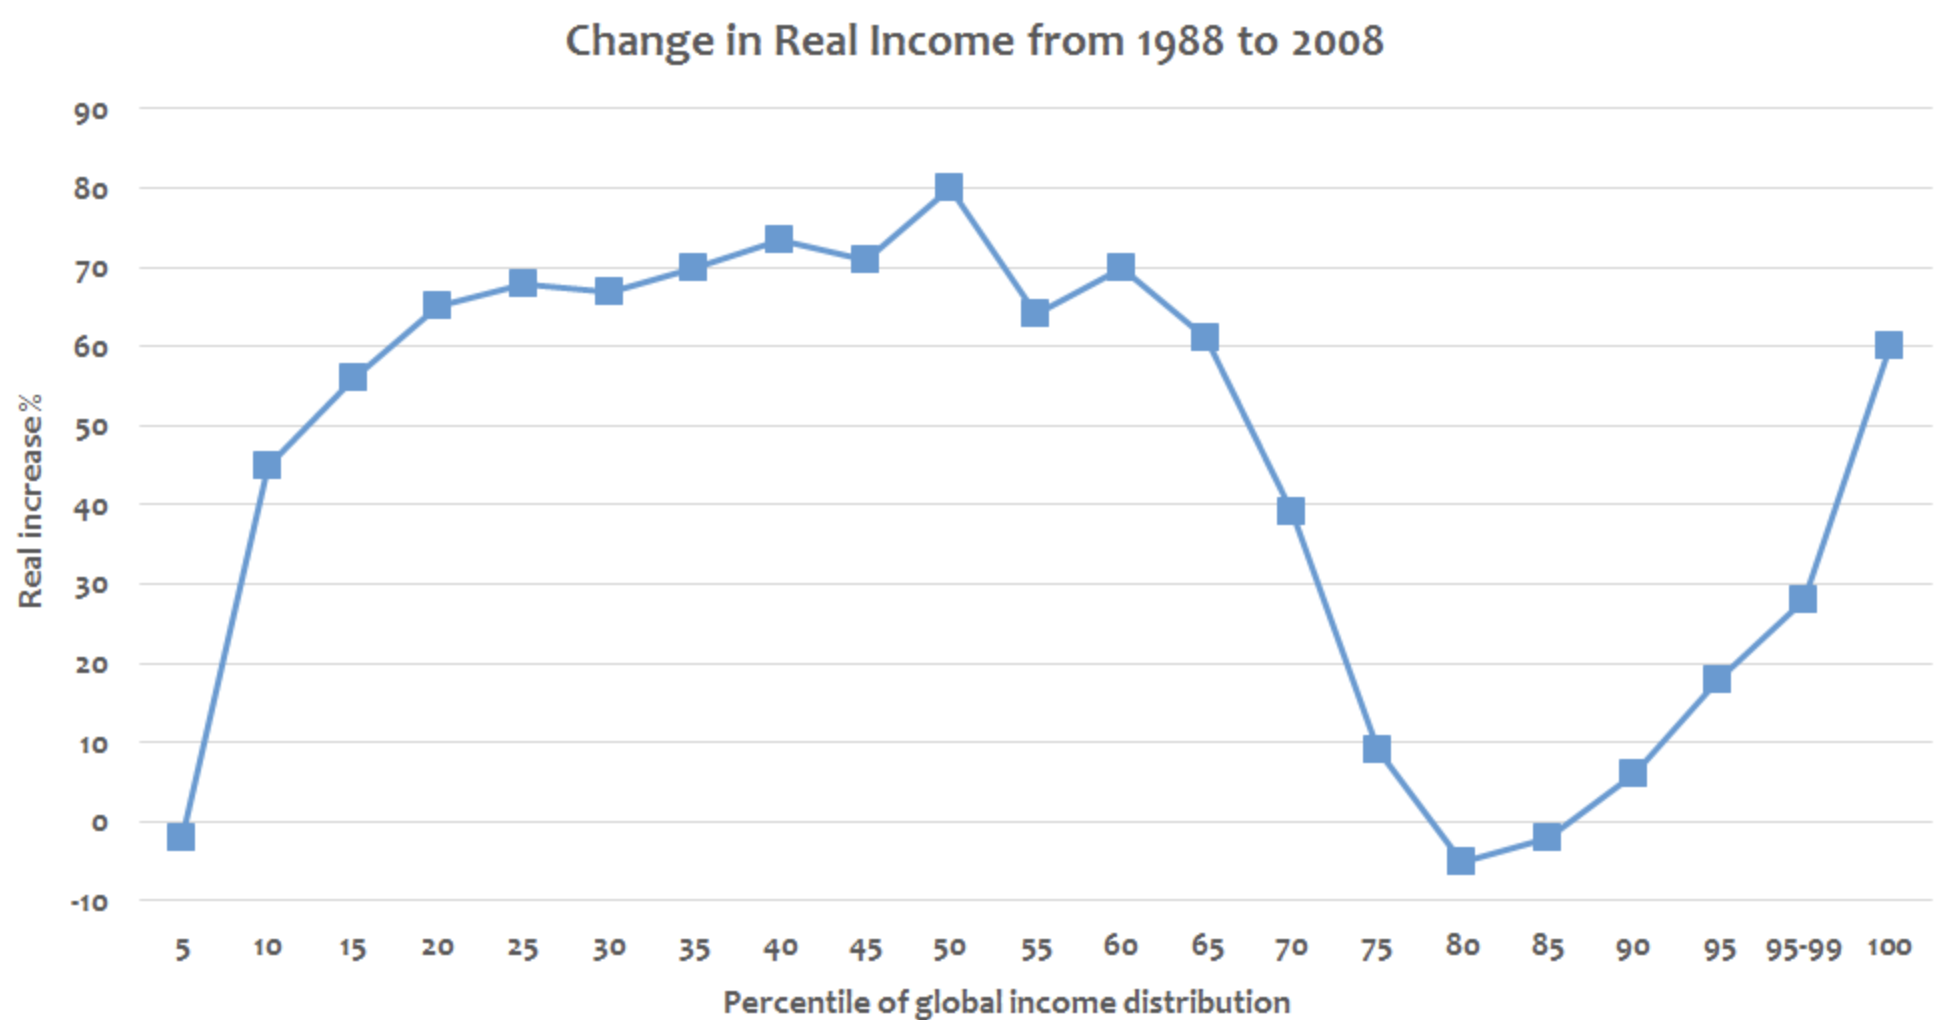
\includegraphics[width = \textwidth]{../img/elephant_milanovic}

\end{frame}
% ----------------------------------------------------
\note{El gráfico del elefante de Branko Milanovic (2012) es quizá la visualización más influyente de la economía política reciente. Muestra quién ha ganado y quién ha perdido con la globalización entre 1988 y 2008. Los grandes ganadores: clases medias de Asia (China, India, Indonesia) y el top 1\% global. Los grandes perdedores: clases medias-bajas de países ricos cuyos ingresos apenas han crecido. Esta estructura ayuda a entender el Brexit, Trump, el auge de extrema derecha en Europa: no es irracionalidad, es respuesta a décadas de estancamiento. Conexión con Rodrik y su trilema de la globalización.}

% ----------------------------------------------------
\begin{frame}
\frametitle{El ``gráfico del elefante'' de Milanovic}
\centering

\begin{itemize}
  \item<1-> Ganadores de la globalización (1988--2008):
  \begin{itemize}
    \item Clases medias asi\'aticas (percentiles 40--60)
    \item Top 1\% global
  \end{itemize}
  \vspace{6pt}
  \item<2-> Perdedores:
  \begin{itemize}
    \item Clases medias-bajas occidentales (percentiles 75--90)
    \item Trabajadores industriales de EEUU, RU, Francia
  \end{itemize}
  \vspace{6pt}
  \item<3-> \alert{Explicación económica} de un fenómeno \textbf{político}: populismo, Brexit, Trump
\end{itemize}
\end{frame}
% ----------------------------------------------------
\note{El gráfico del elefante de Branko Milanovic (2012) es quizá la visualización más influyente de la economía política reciente. Muestra quién ha ganado y quién ha perdido con la globalización entre 1988 y 2008. Los grandes ganadores: clases medias de Asia (China, India, Indonesia) y el top 1\% global. Los grandes perdedores: clases medias-bajas de países ricos cuyos ingresos apenas han crecido. Esta estructura ayuda a entender el Brexit, Trump, el auge de extrema derecha en Europa: no es irracionalidad, es respuesta a décadas de estancamiento. Conexión con Rodrik y su trilema de la globalización.}

% ----------------------------------------------------
\begin{frame}
\frametitle{La reacción populista}
\centering

\begin{columns}[T]
\begin{column}{0.47\textwidth}
\textcolor{accent2}{\textbf{Populismo de derecha}}
\begin{itemize}
  \setlength{\itemsep}{5pt}
  \item Anti-inmigración
  \item Nacionalismo cultural
  \item Proteccionismo
  \item Trump, Brexit, Le Pen, Meloni
\end{itemize}
\end{column}
\begin{column}{0.47\textwidth}
\textcolor{accent}{\textbf{Populismo de izquierda}}
\begin{itemize}
  \setlength{\itemsep}{5pt}
  \item Anti-élites económicas
  \item Redistribución
  \item Crítica a la austeridad
  \item Podemos, Syriza, Sanders
\end{itemize}
\end{column}
\end{columns}

\vspace{10pt}
\onslide<2->{\centering\small Ambos: desconfianza en \textbf{élites} y \textbf{instituciones}}
\end{frame}
% ----------------------------------------------------
\note{El populismo no es uniforme. Derecha: define al pueblo en términos culturales/étnicos; amenaza = inmigrantes y OOII. Izquierda: define al pueblo en términos económicos; amenaza = élites financieras. Ambos desconfían de OOII pero por razones opuestas. Para la política mundial, el populismo de derecha es más directamente desestabilizador: Trump retiró a EEUU de París, impuso aranceles, cuestionó la OTAN.}

% ----------------------------------------------------
\begin{frame}
\frametitle{Migración: el desafío sin gobernanza}
\centering

\begin{itemize}
  \item<1-> $\sim$280 M migrantes internacionales (3{,}6\% población mundial)
  \vspace{6pt}
  \item<2-> Economía: ganancias netas (remesas $>$ ayuda al desarrollo)
  \vspace{6pt}
  \item<3-> Política explosiva:
  \begin{itemize}
    \item Costes/beneficios desigualmente distribuidos
    \item Dimensión identitaria y cultural
    \item Bandera del populismo de derecha
  \end{itemize}
  \item<4-> Efecto de futuros conflictos o cambio climático?
  \vspace{6pt}
  \item<5-> \alert{Problema:} sin gobernanza global comparable a OMC o FMI
\end{itemize}
\end{frame}
% ----------------------------------------------------
\note{La migración es quizá el tema más políticamente explosivo y el que carece de instituciones globales. Los bienes tienen la OMC; el capital, el FMI; las personas, nada comparable. Economía: genera ganancias netas; remesas superan la ayuda al desarrollo. Pero tiene dimensión identitaria que el comercio no tiene. Por eso es la bandera nº 1 del populismo de derecha.}

% ----------------------------------------------------
\begin{frame}
\frametitle{Gaza y el fracaso de R2P}
\centering

\begin{itemize}
  \item<1-> \textbf{Responsabilidad de Proteger (2005):} principio aprobado en la ONU tras Ruanda y Bosnia
  \vspace{6pt}
  \item<2-> Crisis humanitarias 2022--2026: Ucrania, Gaza, Sudán, Myanmar
  \vspace{6pt}
  \item<3-> R2P en la práctica:
  \begin{itemize}
    \item Veto en el Consejo de Seguridad
    \item Doble rasero según alianzas
    \item CPI: órdenes contra líderes, escaso cumplimiento
  \end{itemize}
  \vspace{6pt}
  \item<4-> \alert{Percepción creciente:} el orden liberal tiene un doble estándar
\end{itemize}
\end{frame}
% ----------------------------------------------------
\note{R2P fue uno de los grandes logros normativos de 2005: la idea de que la soberanía implica responsabilidad y que la comunidad internacional puede intervenir ante atrocidades. En la práctica, el mecanismo depende del Consejo de Seguridad y por tanto del veto. Gaza desde 2023 ha puesto esto en evidencia de forma brutal: desde el Sur global, el contraste con la respuesta occidental a Ucrania parece un doble rasero. Esto erosiona la legitimidad del orden liberal y facilita el argumento chino y ruso de que el orden es hipócrita. Conexión con tema 06 (normas, DDHH, derecho internacional humanitario).}

% ----------------------------------------------------
\begin{frame}
\frametitle{ONU, OMC, OMS: instituciones bajo presión}
\centering

\begin{itemize}
  \item<1-> \textbf{ONU:} Consejo de Seguridad paralizado (vetos sistemáticos)
  \vspace{6pt}
  \item<2-> \textbf{OMC:} sin órgano de apelación funcional desde 2019
  \vspace{6pt}
  \item<3-> \textbf{OMS:} salida y reentrada de EEUU, acuerdo sobre pandemias...
  \vspace{6pt}
  \item<4-> \textbf{OTAN:} reactivada por Ucrania, muy cuestionada por EEUU
\end{itemize}

\vspace{8pt}
\onslide<5->{\small \textit{Qué va a pasar: reforma, sustitución o erosión lenta?}}
\end{frame}
% ----------------------------------------------------
\note{Las instituciones del orden liberal están todas bajo presión simultánea. Consejo de Seguridad paralizado por vetos de Rusia/China/EEUU. OMC sin órgano de apelación desde 2019 (Trump bloqueó nombramientos, Biden no los desbloqueó). OMS debilitada por pandemia y por salida/reentrada de EEUU. OTAN paradójicamente más fuerte tras Ucrania, pero cuestionada por la segunda administración Trump. La pregunta clave: ¿se reforman, se sustituyen por alternativas (BRICS+, SCO), o simplemente se vacían de contenido?}

% ----------------------------------------------------
\begin{frame}
\frametitle{Está en crisis el orden internacional?}
\centering

\begin{columns}[T]
\begin{column}{0.47\textwidth}
\textcolor{accent2}{\textbf{Sí}}
\begin{itemize}
  \setlength{\itemsep}{5pt}
  \item Populismo desde dentro
  \item OOII bloqueadas
  \item Doble rasero visible
  \item Rearme y bloques
\end{itemize}
\end{column}
\begin{column}{0.47\textwidth}
\textcolor{accent}{\textbf{No}}
\begin{itemize}
  \setlength{\itemsep}{5pt}
  \item Sin alternativa coherente
  \item OTAN fortalecida
  \item Comercio sigue alto
  \item Normas internalizadas
\end{itemize}
\end{column}
\end{columns}

\vspace{15pt}
\onslide<2->{\centering\small \textit{Reminder: mundo post-1945, DDHH, derecho internacional}}
\end{frame}
% ----------------------------------------------------
\note{Balance. Pesimistas: el orden liberal está en crisis simultánea externa (Rusia, China) e interna (populismo); las instituciones están paralizadas; el doble rasero visible mina la legitimidad. Optimistas: no hay alternativa coherente (BRICS+ no tiene visión común); OTAN se ha fortalecido tras Ucrania; el comercio global sigue siendo alto; muchas normas (prohibición tortura, genocidio) están internalizadas. Respuesta matizada: el orden está cambiando, no colapsando. Emerge un sistema más multipolar, menos liberal, con instituciones debilitadas pero no sustituidas.}

% ====================================================
\section{Nuevas fronteras o problemas: nuclear, cyber, AI}
% ====================================================

% ----------------------------------------------------
\begin{transitionframe}
Nuevas fronteras o problemas: nuclear, cyber, AI
\end{transitionframe}
% ----------------------------------------------------
\note{}

% ----------------------------------------------------
\begin{frame}
\centering
\vspace{2em}
{\large Tres tecnolog\'\i as. Tres formas muy distintas\\
en que el poder y la violencia se reorganizan.}
\end{frame}
% ----------------------------------------------------
\note{Planteamiento. Tres tecnologías con dinámicas muy diferentes: armas nucleares (viejas pero resurgen), cyber (ya aquí, sin reglas claras), IA (emergente, potencialmente transformadora). Cada una plantea un problema distinto de gobernanza internacional.}

% ----------------------------------------------------
\begin{frame}
\frametitle{Disuasión nuclear: ¿sigue funcionando?}
\centering

\begin{itemize}
  \item<1-> \textbf{MAD:} si A ataca, B responde con un segundo golpe $\to$ nadie ataca
  \vspace{6pt}
  \item<2-> Condiciones de funcionamiento:
  \begin{itemize}
    \item Capacidad de segundo golpe
    \item Racionalidad de los líderes
    \item Verificabilidad mutua
  \end{itemize}
  \vspace{6pt}
  \item<3-> 2026: señales preocupantes
  \begin{itemize}
    \item Amenazas rusas en Ucrania
    \item China triplica su arsenal ($\sim$500 cabezas)
    \item EEUU, Israel
    \item Fin de tratados de control (New START expiró en Feb 26)
    \item Rol de la guerra de Irán
  \end{itemize}
\end{itemize}
\end{frame}
% ----------------------------------------------------
\note{La disuasión nuclear ha mantenido la paz entre grandes potencias 80 años. Pero en 2026 se acumulan señales inquietantes. Rusia ha hecho amenazas nucleares explícitas sobre Ucrania. China, que históricamente tenía un arsenal mínimo ($\sim$200 cabezas), se acerca a 500 camino de 1.000. Los tratados de control de armas se desmantelan: INF muerto, New START en vilo. El régimen construido durante la Guerra Fría se erosiona sin reemplazo.}

% ----------------------------------------------------
\begin{frame}
\frametitle{TNP: sigue aguantando?}
\centering

\begin{columns}[T]
\begin{column}{0.47\textwidth}
\textcolor{accent}{\textbf{Éxitos}}
\begin{itemize}
  \setlength{\itemsep}{5pt}
  \item 191 Estados parte
  \item 9 Estados nucleares (no 25)
  \item Sudáfrica, Argentina, Brasil renunciaron
  \item Inspecciones OIEA
\end{itemize}
\end{column}
\begin{column}{0.47\textwidth}
\textcolor{accent2}{\textbf{Fracasos}}
\begin{itemize}
  \setlength{\itemsep}{5pt}
  \item India, Pakistán, Israel nunca firmaron
  \item Corea del Norte salió (2003)
  \item Irán: programa activo? futuro?
  \item Los P5 (permanentes ONU) no desarman
\end{itemize}
\end{column}
\end{columns}

\end{frame}
% ----------------------------------------------------
\note{TNP: uno de los regímenes más exitosos pero con fallas espectaculares. En los 60 se preveían 25+ Estados nucleares; hay 9. Pero los fallos son graves: NK se retiró, Irán mantiene programa activo, el JCPOA de 2015 colapsó con la salida de Trump en 2018. En 2024--2026 Irán ha enriquecido uranio a niveles próximos al militar; Israel ha atacado instalaciones. Si Irán se nucleariza, Arabia Saudí y Turquía probablemente seguirán. Corea del Norte ya tiene $\sim$50 cabezas. La proliferación puede acelerarse.}

% ----------------------------------------------------
\imageframe{../img/ai_dangerous}
\note{}
% ----------------------------------------------------

% ----------------------------------------------------
\begin{frame}
\frametitle{Ciberamenazas}
\centering

\begin{itemize}
  \item<1-> \textbf{Características únicas} de las ciberarmas:
  \begin{itemize}
    \item Atribución difícil
    \item Actores no estatales con gran capacidad
    \item Bajo coste de entrada
  \end{itemize}
  \vspace{6pt}
  \item<2-> Por qué la disuasión no funciona igual?
  \begin{itemize}
    \item Sin atribución clara $\to$ sin represalia creíble
    \item Zona gris: ¿guerra o espionaje?
  \end{itemize}
\end{itemize}
\end{frame}
% ----------------------------------------------------
\note{Las ciberarmas son fundamentalmente distintas a las convencionales o nucleares. Cuando un misil cae, sabes de dónde viene. Un ciberataque puede tardar meses en atribuirse. Eso rompe la lógica de disuasión. Además, actores no estatales pueden causar daño masivo con pocos recursos. WannaCry afectó a 200.000 ordenadores en 150 países. Y no hay consenso sobre cuándo un ciberataque es un acto de guerra.}


% ----------------------------------------------------
\begin{frame}
\frametitle{Precedentes}
\centering

\begin{itemize}
  \setlength{\itemsep}{8pt}
  \item<1-> \textbf{Stuxnet} (2010): EEUU/Israel destruyen centrifugadoras iran\'\i es sin disparar un tiro
  \item<2-> \textbf{SolarWinds} (2020): Rusia penetra $\sim$18.000 redes, incluidos ministerios EEUU
  \item<3-> \textbf{Ransomware} a hospitales y oleoductos (Colonial Pipeline 2021)
  \item<4-> \textbf{Ciberoperaciones en Ucrania:} wipers rusos y defensa ucraniana asistida por Occidente
\end{itemize}

% \vspace{8pt}
% \onslide<5->{\centering\small \textit{La lógica de la disuasión nuclear no se traslada al ciberespacio}}
\end{frame}
% ----------------------------------------------------
\note{Cuatro casos que muestran la evolución del ciberconflicto. Stuxnet (2010): primer caso documentado de un arma cibernética con efectos físicos (destruir centrifugadoras). SolarWinds (2020): ataque de cadena de suministro masivo atribuido a Rusia; compromiso masivo sin respuesta clara. Colonial Pipeline (2021): ransomware paralizó el suministro de combustible en el este de EEUU. Ucrania desde 2022: primer conflicto donde el cyber acompaña a las operaciones militares; Rusia usa wipers, Ucrania recibe apoyo cibernético masivo de aliados y de empresas (Microsoft, Starlink).}

% ----------------------------------------------------
\begin{frame}
\frametitle{La próxima carrera geopolítica?}
\centering

\begin{itemize}
  \item<1-> La \textbf{inteligencia artificial} y su desarrollo muy rápido
  \item<1-> Dimensión militar: armas autónomas, drones, ciberdefensa
  \item<1-> Dimensión económica: productividad, automatización
  \item<2-> Dimensión geopolítica:
  \begin{itemize}
    \item Control de semiconductores (EEUU vs China)
    \item Modelos dominantes (OpenAI, Anthropic, DeepSeek\dots)
    \item \alert{Sin gobernanza internacional}
  \end{itemize}
\end{itemize}
\end{frame}
% ----------------------------------------------------
\note{La IA es posiblemente la tecnología más transformadora del siglo XXI y ya es campo de competición geopolítica. Militar: armas autónomas plantean problemas éticos y legales (el derecho humanitario exige decisión humana en el uso de la fuerza). Económica: amplía la brecha entre los que adoptan y los que no; el desarrollo se concentra en EEUU y China. Geopolítica: la cadena de semiconductores (TSMC, ASML, NVIDIA) es el nuevo cuello de botella instrumentalizado (CHIPS Act, restricciones de exportación). A diferencia del nuclear (TNP) o el clima (París), no hay gobernanza global de la IA.}

% ----------------------------------------------------
\begin{frame}
\frametitle{Qué pasa con los nuevos desarrollos?}
\centering

\begin{columns}[T]
\begin{column}{0.47\textwidth}
\textcolor{accent2}{\textbf{Inestabilidad}}
\begin{itemize}
  \setlength{\itemsep}{5pt}
  \item Sin reglas claras
  \item Actores no estatales
  \item Tecnolog\'\i a m\'as r\'apida que regulaci\'on
  \item Proliferaci\'on nuclear
\end{itemize}
\end{column}
\begin{column}{0.47\textwidth}
\textcolor{accent}{\textbf{Nada nuevo}}
\begin{itemize}
  \setlength{\itemsep}{5pt}
  \item Los Estados aprenden
  \item Aparecen normas informales
  \item Interés mutuo en evitar catástrofe
  \item El TNP se consiguió
\end{itemize}
\end{column}
\end{columns}

\end{frame}
% ----------------------------------------------------
\note{Balance. Pesimistas: el ritmo tecnológico supera a la regulación; actores no estatales aumentan su capacidad destructiva; el régimen nuclear se erosiona. Optimistas: los Estados acabaron regulando lo nuclear tras Hiroshima y varias crisis; normas informales emergen (tabú de armas biológicas, prohibición informal de ataques a civiles en cyber); el interés mutuo en evitar catástrofes puede producir cooperación tardía. Respuesta matizada: en todas las tecnologías pasadas ha habido un lag entre capacidad y regulación, pero al final se regulan; la pregunta es cuántas catástrofes hacen falta para que ocurra.}

% ====================================================
\section{Cierre}
% ====================================================

% ----------------------------------------------------
\begin{transitionframe}
Todo está conectado
\end{transitionframe}
% ----------------------------------------------------
\note{}

% % ----------------------------------------------------
% \begin{frame}
% \frametitle{Todo conecta: Intereses, Interacciones, Instituciones}
% \centering
% \vspace{0.3em}

% \scriptsize
% \begin{tabularx}{\textwidth}{>{\bfseries}l L L L}
%  & \textbf{Intereses} & \textbf{Interacciones} & \textbf{Instituciones} \\[3pt]
% \hline
% D1 Guerra GP & Poder, seguridad & Bargaining, Tuc\'\i dides & OTAN, ONU, disuasi\'on \\[4pt]
% D2 Bienes p\'ublicos & Aire limpio, nadie paga & Dilema del prisionero global & Montreal, Par\'\i s, OMS \\[4pt]
% D3 Globalizaci\'on & Ricardo vs.~seguridad & Weaponized interdep. & OMC, sanciones, CHIPS Act \\[4pt]
% D4 Orden liberal & Comercio, DDHH vs.~soberan\'\i a & Populismo, migraci\'on & ONU, OMC, R2P \\[4pt]
% D5 Nuevas fronteras & Seguridad, ventaja tec. & Disuasi\'on, carrera & TNP, OIEA, sin gobernanza IA \\[3pt]
% \end{tabularx}
% \end{frame}
% % ----------------------------------------------------
% \note{Slide de síntesis. Los cinco debates se pueden leer con el marco I--I--I. Guerra entre grandes potencias: intereses de poder/seguridad, interacción tipo Tucídides, instituciones como OTAN y disuasión. Bienes públicos: intereses divergentes, dilema del prisionero, instituciones como París. Globalización: intereses económicos vs. seguridad, weaponized interdependence, OMC y CHIPS Act. Orden liberal: tensión entre valores universales y soberanía, reacción populista, instituciones bajo presión. Nuevas fronteras: seguridad y ventaja tecnológica, carrera y disuasión, TNP funcional pero sin equivalente para cyber e IA. Este marco es lo más valioso del curso.}

% ----------------------------------------------------
\begin{frame}
\frametitle{Conexiones}
\centering

\begin{itemize}
  \setlength{\itemsep}{6pt}
  \item<1-> \textbf{Taiwán:} guerra GP + decoupling + semiconductores + IA + drones...
  \item<3-> \textbf{Clima:} cooperación + Norte--Sur + globalización tecnológica
  \item<4-> \textbf{AI:} nuevas fronteras + globalización + competencia EEUU--China + guerra autónoma...
\end{itemize}

\end{frame}
% ----------------------------------------------------
\note{Los cinco debates no son independientes. Taiwán junta cuatro: guerra entre grandes potencias, decoupling, cadena de semiconductores, carrera de IA. Ucrania junta guerra GP, sanciones (weaponized interdependence), desafío al orden liberal, y amenazas nucleares. El clima cruza cooperación, Norte--Sur y competencia tecnológica (quién lidera en renovables). La IA está en el centro de varios debates. Ver el tablero completo es ver una sola red.}

% ----------------------------------------------------
\begin{frame}
\centering
\vspace{2em}
{\large De los cinco debates, \textbf{cuál definirá m\'as\\ los próximos 10 años?}}

\end{frame}
% ----------------------------------------------------
\note{Pregunta final abierta. Invitar a los estudiantes a elegir y justificar. No hay respuesta correcta. Guiar: si eligen guerra GP, preguntar por Taiwán; si eligen clima, por Norte--Sur; si eligen globalización, por sanciones; si eligen orden liberal, por populismo; si eligen tecnología, por IA y cyber. Valorar justificaciones que usen el marco del curso.}

% ----------------------------------------------------
\begin{frame}
\centering
\vspace{3em}
{\large ¿Preguntas?}

\end{frame}
% ----------------------------------------------------
\note{Slide final. Agradecer la participación durante el curso. Abrir a preguntas libres sobre cualquier tema del curso o sobre la clase de hoy. Recordar fechas del examen y temas que entran. Indicar que todos los materiales están en la web del curso.}
